\documentclass[a4paper,headsepline,bibliography=totoc]
							{scrartcl}
\usepackage[english]{babel}
\usepackage{graphicx}
\usepackage{makeidx}
\usepackage[utf8]{inputenc}
\usepackage{textgreek}
\usepackage{amsmath}
\usepackage{amssymb}
\usepackage{bigstrut}
\usepackage[center,font=footnotesize]{caption}
\usepackage{geometry}
\usepackage{pdfpages}
\usepackage{epstopdf}
\usepackage{multicol}
\usepackage{listings}
\usepackage{color}
\usepackage[ruled,vlined,linesnumbered]{algorithm2e} % pseudocode layout
\usepackage{booktabs} % beautiful tables
\usepackage[centerlast]{subfigure}
\usepackage{url}
\usepackage[section]{placeins} 		% 	Paket für erweiterte 													Positionierung von 													Gleitobjekten, Gleitobjekte 										dürfen Abschnitt nicht verlassen
%\usepackage[nottoc]{tocbibind}
\usepackage{caption}
\usepackage[automark]{scrlayer-scrpage}
\usepackage[
    linktocpage=true,
    bookmarksopenlevel=section]
    {hyperref}
%\usepackage{lmodern}
%\usepackage{latexsym}
%++++++++++++++++++++++++++++++++++++++++++++++++++++++++++% Bibi
\usepackage[babel, german=quotes]{csquotes}
					% Stil der Zitate und der Bibliographie
\usepackage[style=alphabetic,backend=biber,
bibencoding=utf8, natbib=true
]{biblatex}
\addbibresource{Bib.bib} % <---
%++++++++++++++++++++++++++++++++++++++++++++++++++++++++++%
\geometry{a4paper,left=30mm,right=30mm, top=3cm, bottom=3cm}
\graphicspath{{images/}} 					% legt globalen Pfad für 													Bilddateien fest
%\makeatletter 										% Legt fest das 														nach Chapter nicht
\newcommand{\ra}[1]{\renewcommand{\arraystretch}{#1}}
%\makeatother											% zwingend 													einen neue seite anfängt
% BEGIN Settings for code-listings

\definecolor{mygreen}{rgb}{0,0.6,0}
\definecolor{mygray}{rgb}{0.5,0.5,0.5}
\definecolor{mymauve}{rgb}{0.58,0,0.82}

\lstset{
  backgroundcolor=\color{white},   % choose the background color; you must add \usepackage{color} or \usepackage{xcolor}; should come as last argument
  basicstyle=\footnotesize,        % the size of the fonts that are used for the code
  breakatwhitespace=false,         % sets if automatic breaks should only happen at whitespace
  breaklines=true,                 % sets automatic line breaking
  captionpos=b,                    % sets the caption-position to bottom
  commentstyle=\color{mygreen},    % comment style
  deletekeywords={...},            % if you want to delete keywords from the given language
  extendedchars=true,              % lets you use non-ASCII characters; for 8-bits encodings only, does not work with UTF-8
  firstnumber=1,                % start line enumeration with line 1
  frame=single,                    % adds a frame around the code
  keepspaces=true,                 % keeps spaces in text, useful for keeping indentation of code (possibly needs columns=flexible)
  keywordstyle=\color{blue},       % keyword style
  language=R,                 % the language of the code
  morekeywords={*,...},            % if you want to add more keywords to the set
  numbers=left,                    % where to put the line-numbers; possible values are (none, left, right)
  numbersep=7pt,                   % how far the line-numbers are from the code
  numberstyle=\color{black}, % the style that is used for the line-numbers
  rulecolor=\color{black},         % if not set, the frame-color may be changed on line-breaks within not-black text (e.g. comments (green here))
  showspaces=false,                % show spaces everywhere adding particular underscores; it overrides 'showstringspaces'
  showstringspaces=false,          % underline spaces within strings only
  showtabs=false,                  % show tabs within strings adding particular underscores
  stepnumber=1,                    % the step between two line-numbers. If it's 1, each line will be numbered
  stringstyle=\color{mymauve},     % string literal style
  tabsize=2,                     % sets default tabsize to 2 spaces
  title=\lstname                   % show the filename of files included with \lstinputlisting; also try caption instead of title
}
% END Settings for code-listings
\sloppy
\setlength{\parindent}{0mm}
%+++++++++++++++++++++++++++++++++++++++++++++++++++++++++++%
\pagestyle{scrheadings}
\ihead[]{\today} %- linke Kopfzeile
\chead[]{\versuchkurz} %- mittlere Kopfzeile
\ohead[]{\rightmark} %- rechte Kopfzeile
\ifoot[]{} %- linke Fußzeile
\cfoot[]{\pagemark} %- mittlere Fußzeile
\ofoot[]{} %- rechte Fußzeile
% !Tex root = Vorlage.tex
\newcommand{\versuch}{A Robust Approach for Discovering Functional Dependencies using Machine Learning Approaches}
\newcommand{\student}{Philipp Jung}
\newcommand{\versuchkurz}{MLFD}
\newcommand{\supervisor}{Prof. Felix Biessmann}
\newcommand{\supervisortwo}{Dr. Zweit Gutachterin}
\newcommand{\datumversuch}{16.03.2019}
\newcommand{\matrnr}{872855}

%+++++++++++++++++++++++++++++++++++++++++++++++++++++++++++%
\begin{document}
\setcounter{page}{0}
% !Tex root = main.tex
\begin{titlepage}
  \begin{figure}[h]
      \begin{flushright}
      
\includegraphics[width=.4\textwidth]{images/beuth-logo.png}
      \end{flushright}
    \label{fig:spektren01sd}
  \end{figure}

  \vspace{10mm}

  \begin{center}
    \vspace{10mm}
    {Master's Thesis\\}
    \vspace{10mm}
    {\Huge \versuch \\}
    \vspace{15mm}
    {by\\}
    \vspace{3mm}
    {\student}\\
    \vspace{15mm}
    {\footnotesize Business Administration and Engineering - Project Management M.A.\\}
    {\footnotesize Fachbereich I}
  \end{center}

  \vfill
  \parbox[t]{0.45\textwidth}{
      {\student}\\
      Matriculation Number: {\matrnr}\\
      \datumversuch
    }%
  \hfill
  \begin{tabular}[t]{l@{}}%{\raggedleft
  Advisors:\\
    {\supervisor}\\
    {\supervisortwo}
  \end{tabular}
\end{titlepage}

\pagenumbering{Roman}
ABSTRACT. Lorem ipsum dolor sit amet, consetetur sadipscing elitr, sed diam nonumy eirmod
tempor invidunt ut labore et dolore magna aliquyam erat, sed diam voluptua. At
vero eos et accusam et justo duo dolores et ea rebum. Stet clita kasd gubergren,
no sea takimata sanctus est Lorem ipsum dolor sit amet.

\newpage
\newpage
\tableofcontents
\newpage
\pagenumbering{arabic}
\linespread{1.5}
% !Tex root = main.tex
\section{Introduction}
Data-driven methods change the way computer scientists approach algorithmic problems.
Rather than designing and implementing complex algorithms themselves, recent advances in machine learning have allowed for learned algorithms.

Kraska et al.\ showed in their 2018 publication ``The case for Learned Index Structures'' that different index structures can be replaced by learned ones, greatly improving performance.~\cite{KRA18}
In the field of data cleaning and data enrichment, HoloClean lead the way for machine-learning approaches in the domain of data cleaning.~\cite{HEI19}
HoloClean is agnostic of the way data is structured, making it versatile for many different domains of application.

In this work, machine-learning techniques are applied to the field of relational database theory --- more precisely, functional dependency detection.
Stemming from the beginnings of relational database theory, functional dependencies were introduced to formalize normalization of relational schemata.

In the theoretical part of this thesis, the basic relational database terminology is introduced.
Furthermore, limitations of canonical functional dependencies are mentioned and relaxed functional dependencies are introduced.
With reference to Koudas et al., functional dependencies' robustness is discussed.
A method for measuring robustness is proposed.
Mean square error and F1-Score are introduced to measure the performance of imputation models.

Machine-learning classification theory necessary for understanding the basic functionality of the Datawig framework~\cite{BIE18} is discussed.
It is described how robustness of FDs is measured using an algorithm called FD Imputer.
FD Imputer's machine-learning counterpart, called ML Imputer, is presented.
The theoretical part of this thesis is concluded with a discussion of how to detect dependencies using learned imputation models using an algorithm called DepDetector.

Several experiments are conducted to explore machine-learning techniques applied to functional dependency analysis.
FD Imputer is run on a range of datasets and FDs are ranked according to their robustness.
The experiment is repeated with ML Imputer.
ML Imputer is overfitted and implications of overfitting on the FD robustness-ranking are examined.
The final building block of the experimental section is formed by dependency detection with DepDetector.

Results are discussed and recommendations for future research in learned dependency detection are issued in the final section of this work.

% !Tex root = main.tex
\newpage
\section{Theory}
\emph{Functional Dependencies}(FDs) are a way of expressing ``a priori knowledge of restrictions or constraints on permissible sets of data''~\cite[p.~42]{MAI83} in relational database theory.
Since first work in the 1970s on schema normalization has been done, FDs have proven to be very useful for schema normalization.


\subsection{Relational Database Theory}
In order to give a definition of FDs, they need to be put in context to the domain they stem from: relational database theory. Some basic concepts will be introduced in this section.


\subsubsection{Relation Scheme}
A \emph{relation scheme}\footnote{also called \emph{relational schema} in literature\cite[p.21]{ABE19} } \(\boldsymbol{R}\) is a finite set of \emph{attribute names} \(\{A_1, A_2, \dots, A_n\}\), where to each attribute name \(A_i\) corresponds a set \(D_i\), called \emph{domain} of \(A_i\), \(1 \leq i \leq n\).
Let \(\boldsymbol{D} = D_1 \cup D_2 \cup \dots \cup D_n$, then a \emph{relation} \(r\) on relation scheme \(\boldsymbol{R}\) is a finite set of mappings \(\{t_1, t_2, \dots, t_p\}\) from \(\boldsymbol{R}\) to \(\boldsymbol{D}\):

\begin{align*}
  &t_i: \boldsymbol{R} \to \boldsymbol{D},
\end{align*}

where we call those mappings \emph{tuples} under the constraint that~\cite[p.2]{MAI83}

\begin{align*}
    t(A_i) \subseteq D_i.
\end{align*}

In application, attribute names are commonly called \emph{column name} or \emph{column attribute}.
One can think of them as labels of data that is stored in the respective column.


\subsubsection{Keys}
A \emph{key} on a relation \( r \) on a relation scheme \( R \) is a subset \( K = \{ B_1, B_2, \dots, B_m \} \) with the property that for any tuple \( t_i \in \{ t_1, t_2, \dots, t_3 \} \) the relation

\begin{align*}
    t_i(B_k) = t_j(B_k) \Rightarrow t_i \equiv t_j
\end{align*}

holds for any single \( B_k \in K \). In other words, any \( K \)-value of a tuple identifies that tuple uniquely.~\cite[p.~4]{MAI83} \\

Having defined both \emph{ralation scheme} and \emph{keys}, it is now possible to introduce the more complex conepts of \emph{relational databases} and \emph{functional dependencies}.


\subsubsection{Definition of a Relational Database}
When real-world data used by one or multiple application/s is stored on a machine according to the relational model, it is usually stored in a relational database.
According to the definition of a relation scheme \(R\), one can formally introduce databases and database schemes: \\

We assume that \(R\) is composed of two parts, \(S\) and \(\boldsymbol{K}\). We call \(S\) a \emph{set of attributes} and \(\boldsymbol{K}\) a \emph{set of designated keys} and describe this composition by writing \(R = (S, \boldsymbol{K})\).
A \emph{relational database scheme} \textbf{R} over \textbf{U} can now be defined as a collection of relation schemes \(\{R_1, R_1, \dots, R_p\}\), where \(R_i = (S_i, \boldsymbol{K}_i)\), \(1 \leq i, j \leq p\),

\begin{align*}
    \bigcup^{p}_{i=1} S_i = \boldsymbol{U}.
\end{align*}

We demand that \(S_i \neq S_j\) if \(i \neq j\). \\

A \emph{relational database} \( d \) on a \emph{database scheme} \textbf{R} is a collection of relations \( d~=~\{r_1, r_2, \dots, r_p \} \) such that for each relation scheme \(R = (S, \boldsymbol{K}) \) in \textbf{R} there is a relation \(r\) in \(d\) such that \(r\) is a relation on \(S\) that satisfies every \emph{key} in \(\boldsymbol{K}\).~\cite[p.~94]{MAI83}


\subsubsection{Definition of a Functional Dependency}
Consider a relation \(r\) on scheme \(\boldsymbol{R}\) with subset \(X \subseteq \boldsymbol{R}\) and a single attribute \(A_i \in \boldsymbol{R}\).
A FD \(X \to A\) is said to be \emph{valid} in \(r\), if and only if

\begin{align}
    t_i[X] = t_j[X] \Rightarrow t_i[A] = t_j[A] \label{eq:fd-condition}
\end{align}

holds for all all pairs of distinct tuples \(t_i,t_j \in r\).\cite[p.~21]{ABE19}
We say that \(X\) \emph{functionally determines} \(A\)\cite[p.~43]{MAI83} and name \(X\) the \emph{left side}, whilst calling \(A\) the \emph{right side}.\\

\begin{table}[ht]
    \centering
    \begin{tabular}{lcccc}
        \toprule
        & \multicolumn{3}{c}{left side} & \multicolumn{1}{c}{right side} \\ \cmidrule(lr{.75em}){2-3} \cmidrule(lr{.75em}){4-5}
        ID & FIRST NAME & LAST NAME & TOWN & ZIP \\
        \midrule
        1 & Alice & Smith & Munich & 19139 \\
        2 & Peter& Meyer & Muinch & 19139 \\
        3 & Ana & Parker & Munich & 19139  \\
        4 & John & Pick & Berlin & 12055 \\
        \bottomrule
    \end{tabular}
    \caption{Even though column ZIP functionally determines column Town (and vice-versa), a FD is not capable of displaying this fact - a typing error invalidates the FD.}
    \label{tab:example-afd-necessity}
\end{table}


\section{FDs in Application}
FDs are primarily used in database normalization,\cite[p.~1]{CAR16} but also find application in the field of data profiling, where ``any dependency can be turned into a rule to check for errors in the data''.\cite[p.~9]{ABE19}


\subsection{Normalization}
When introducing the relational database model in his 1970 article ``A relational model of data for large shared data banks'', Edgar F. Codd formalized database normalization alongside.\cite{COD70}
Describing what will be know to academia as \textbf{First normal form} (1NF), Codd states that ``problems treated [when normalizing databases] are those of \emph{data independence}'', aiming to protect future users of large databases ``from having to know how the data is organized in the machine''. \cite[p.~1]{COD70} \\

Being designed for as efficient as possible query handling, databases at the time were structured hierarchically or navigationally.
While this yielded good performance in times when computing time was very expensive, it came with a heavy cost of complexity:
``Teams of programmers were needed to express queries to extract meaningful information. [\dots] Such databases [\dots] were absolutely inflexible[y]''.\cite{IBM03}

Update-, insertion- and deletion anomalies can be prevented when normalizing a relational database. \cite[p.~75]{KLE11}

\subsubsection{First Normal Form}
A relation scheme $R$ is in \emph{First Normal Form} (1NF), if values in \(dom(A)\) are atomic for every attribute \(A\) in \(R\). \cite[p.~96]{MAI83}
Consider table \ref{tab:first-normal-form} which represents two relational database schemes.
It serves as an example of what is called \emph{atomic} and \emph{compound} data in the Relational Database model. \cite[p.~6]{COD90}

\begin{table}[ht]
    \centering
    \ra{1.3}
    \begin{tabular}{@{}rlllllll@{}}\toprule
    & \multicolumn{3}{c}{compound scheme} & \phantom{abc}& \multicolumn{2}{c}{atomic scheme} \\
    \cmidrule{2-3} \cmidrule{5-8}
    & NAME & ADRESS && PRENAME & SURNAME & TOWN & STREET   \\ \midrule
    1 & Alice Smith & Munich, Alicestr. && Alice & Smith & Alicestr. & Munich \\
2 &  Peter Meyer & Munich, Peterstr. && Peter & Meyer & Munich & Peterstr. \\
3 & Ana Parker & Munich, Anastr. && Ana & Parker & Munich & Anastr. \\
4 & John Pick & Berlin, Johnstr. && John & Pick & Berlin & Johnstr. \\
\bottomrule
\end{tabular}
\caption{The compound attributes ADRESS and NAME can be split into their atomic components TOWN and STREET as well as PRENAME and SURNAME, respectively.}
\label{tab:first-normal-form}
\end{table}
While the compound scheme's attributes can be decomposed into several other attributes, whereas an atomic attribute cannot be further split into any meaningful smaller components.\\

For a database it is said that the database in 1NF if every relation scheme in the database scheme is in 1NF.
1NF is the very foundation of the Relational Model, where the only type of compound data is the relation.\cite[p.~6]{COD90}

\subsubsection{Second Normal Form (2NF)}
A relation scheme \(R\) is said to be in \emph{Secon Normal Form} (2NF) in respect to a set of FDs \(F\), if it is in 1NF and every nonprime attribute is fully dependent on every key of of \(R\).\cite[p.~99]{MAI83}

\subsubsection{Third Normal Form (3NF)}

\subsection{Approximate Functional Dependencies}
In the field of data profiling an extensive body of theory and algorithms for FD detection has been created in the past decades.\cite{PAP15}
These mainly consider FDs as defined in formula \ref{eq:fd-condition}.
Howevever, the strict detection of FDs yields results that are solely applicable in a strictly controlled environment.
Real-world datasets faced by data-scientists or database engineers are often \emph{noisy}.
Entries might be corrupted by missing data, wrongly entered entries or incomplete datasets.
Inconsistencies are to be expected.
Thus, functionally dependent column-combinations might not be detected as such. This may result in misleading insights when searching for FDs. \\

To illustrate this, table \ref{tab:example-afd-necessity} shows an example of noisy data.
The potential FD \textbf{Town} \(\to\) \textbf{ZIP} is not captured by the definition given in equation \ref{eq:fd-condition}.
Due to a type-error, the potential FD is invalidated.
To still capture meta-information, a different dependency-measure than given in equation \ref{eq:fd-condition} is needed. \\

\emph{Approximate FDs} (AFDs), sometimes called \emph{Relaxed FDs}, improve the applicability of FDs, ``in that they relax one or more constraints of the canonical FDs''\cite[p.~1]{CAR16}. While there are AFDs introducing general error measures, others are defined ``aiming to solve specific problems''\cite[p.~1]{CAR16}. \\

\begin{table}[ht]
    \centering
    \begin{tabular}{lcccc}
        \toprule
        & \multicolumn{3}{c}{Data} \\ \cmidrule(lr){2-5}
        ID & First name & Last name & Town & ZIP \\
        \midrule
        1 & Alice & Smith & Munich & 19139 \\
        \textbf{2} & \textbf{Peter}& \textbf{Meyer} &
        \textbf{Muinch} & \textbf{19139} \\
        3 & Ana & Parker & Munich & 19139  \\
        4 & John & Pick & Berlin & 12055 \\
        \bottomrule
    \end{tabular}
    \caption{Even though column ZIP functionally determines column Town (and vice-versa), a FD is not capable of displaying this fact - a typing error invalidates the FD.}
    \label{tab:example-afd-necessity}
\end{table}

The error measure for this is not trivial at all. While F1-measures can be established for non-categorical cases, comparing results for different data-types tricky.

\subsection{FD Imputer}


\begin{algorithm}[H]
    \DontPrintSemicolon
    \SetAlgoLined
    \KwResult{Imputed column of a relational database}
    \KwData{Relational database}
    \BlankLine

    Split relational database in test-set and train-set\;
    Detect FDs in train-set\;
    \For{row in test-set}{
        Find row in train-set with equal LHS combination\;
        \If{matching LHS combination found}{
            impute with RHS from train-set\;
        }
        \If{No matching LHS combination found in train-set}{
            impute with NaN\;
        }
    }
    \caption{An imputer operating on Functional Dependencies}
\end{algorithm}

% !Tex root = Vorlage.tex
\newpage
\section{Execution}
A number of experiments have been conducted in order to evaluate the capabilities of empirical risk minimization (ERM) techniques for functional dependency discovery.

All rows containing missing values are dropped due to possible inconsistencies.

\subsection{FD Imputer}
The FD Imputer

\subsection{ML Imputer}

\subsubsection{Overfitting the ML Imputer}

\subsection{Comparing ML Imputer with FD Imputer}
As discussed in the previous section, ML Imputer and FD imputer differ fundamentally in the way they function.
When comparing the two, metrics need to be computed bearing those differences in mind.

The measure chosen to compare imputation performance on columns containing continuous numeric values is the \emph{mean squared error} (MSE).
FD Imputer cannot approximate numerical values.
Due to the nature of the definition of a FD, Data is always assumed to be classifiable.
Meanwhile, ML Imputer is able to perform regression, predicting a continuous label for a given input with an uncertainty.

Naturally, this circumstance leads to a far superior performance of ML Imputer when imputing continuous labels.
FD Imputer usually doesn't find any values on the train set to impute with and cannot return a meaningful result.
Taking the above into account, rows that aren't imputed by FD Imputer are not considered when computing a performance measure on columns containing continuous values.

To compare classification performance, the F1-measure is chosen.

\subsection{Classification Performance}
ML Imputer and FD Imputer were compared on two established Machine Learning datasets, Adult\footnote{\url{https://archive.ics.uci.edu/ml/datasets/adult}} and Nursery\footnote{\url{https://archive.ics.uci.edu/ml/datasets/nursery}}.
Adult's scheme is not normalized.
The table contains 70-something FDs.
In contrast to this, the Nursery dataset is strongly normalized.
It contains a mere 9 FDs, 8 of which are between the scheme's key and each attribute, respectively.

The complementary nature of these two datasets enables the observation of imputer performance in function of the degree of normalization.

\subsection{FD Imputer Performance}
FD Imputer is run for every FD found on a train subset of Adult and Nursery, respectively.
Figure~\ref{fig:f1_fd_adult} shows the performance of FD Imputer on columns containing classifiable data.
\begin{figure}[h]
     \centering
     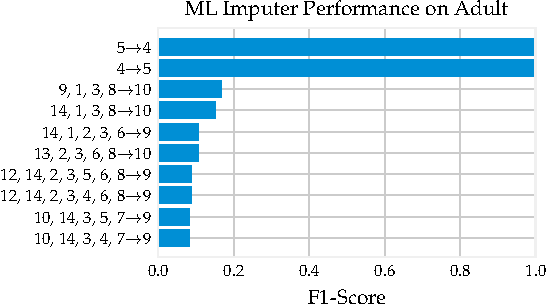
\includegraphics[width=.8\textwidth]{../figures/adult/f1_fd_imputer_adult.pdf}
     \caption{F1 score of the 10 most performant FDs when imputing values on a validation set.}
     \label{fig:f1_fd_adult}
 \end{figure}
The two top performing FDs have a perfect F1 score of 1 each.
An explanation for this can be found when analyzing the content of columns 4 and 5.
Column 4 contains information about the highest educational level achieved.

There are 16 different categories of educational level defined.
Each category is assigned an integer in a range from 0 to 15.
This integer is the content of column 5.
Thus, the relation between column 4 and column 5 can be modeled by a bijective function between the domains of each attribute.

\begin{table}[ht]
    \centering
    \begin{tabular}{lrrrr}
        \toprule
        & & \multicolumn{2}{c}{Performance} &  \\ \cmidrule(lr{.25em}){2-5}
        Dataset & F1\textsubscript{mean} & F1\textsubscript{max} & F1\textsubscript{min} & \(|\text{F1} = 0|\)\\
        \midrule
        adult & 0.0669 & 1.0000 & 0.0000 & 10 \\
        nursery & 0.0000 & 0.0000 & 0.0000 & 10 \\
        \bottomrule
    \end{tabular}
    \caption{Performance of the FD Imputer.}\label{tab:fd-imputer-performance}
\end{table}
Other FDs lead to F1 scores \(< 0.2\), yielding substantially worse results than the top two FDs.
It can be derived that only the two top-performing FDs hold in a general case.
If unseen data is added to the dataset, it can thus safely be assumed that these two FDs still hold.

\begin{figure}[h]
     \centering
     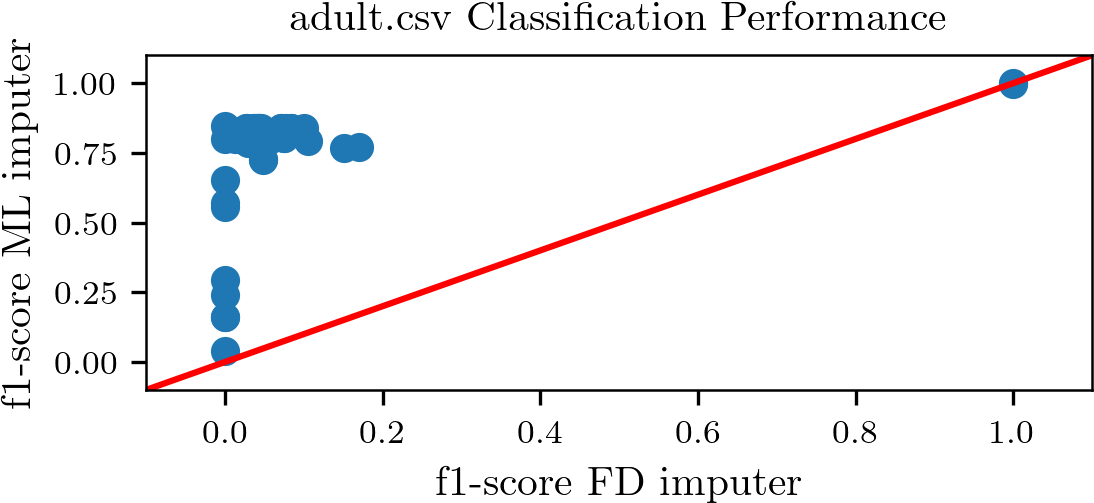
\includegraphics[width=.8\textwidth]{../figures/adult/f1_ml_fd_adult}
     \caption{The figure compares the f1-score of the FD Imputer compared to the f1-score of the ML Imputer. Each point represents one FD.}
     \label{fig:f1_ml_fd_adult}
 \end{figure}

Figure~\ref{fig:f1_ml_fd_adult} compares the F1-scores of both ML Imputer and FD Imputer on the Adult dataset.
One can observe that for most FDs, the ML Imputer performs better than the FD Imputer.
FD Imputer performance and ML Imputer performance seem to be proportional.
If the ML imputer's F1-score is lower than 0.7, the FD Imputer's F1-score for the same FD is 0.
However, for FD's where the ML Imputer scores are larger than 0.7, the FD Imputer scores better than 0.0.
Interestingly, there are two FDs for which the FD Imputer performs equally good or better than the ML Imputer.

The same comparison as
 \begin{figure}[h]
     \centering
     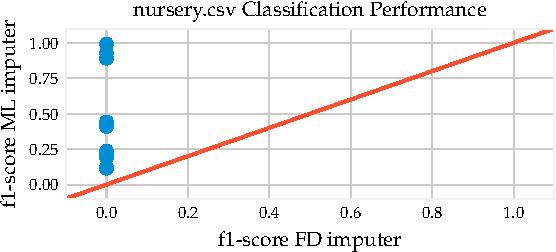
\includegraphics[width=.8\textwidth]{../figures/nursery/f1_ml_fd_nursery}
     \caption{Some ohter caption.}
     \label{fig:f1_ml_fd_nursery}
\end{figure}

\subsection{Begriffsdiskussion}
Lorem ipsum dolor sit amet, consetetur sadipscing elitr, sed diam nonumy eirmod
tempor invidunt ut labore et dolore magna aliquyam erat, sed diam voluptua. At
vero eos et accusam et justo duo dolores et ea rebum. Stet clita kasd gubergren,
no sea takimata sanctus est Lorem ipsum dolor sit amet.

% !Tex root = main.tex
\newpage
\section{Discussion}
\subsection{Robustness}
Robustness is introduced in order to measure the imputation-capabilities of an FD using FD Imputer.
It is successfully demonstrated that FDs with a high robustness also contain humanly explainable meanings, for example when discussing figure~\ref{fig:f1_fd_adult}.

However, it was possible to demonstrate that FDs do not offer any insights about the profile of data.
They are fit for the specific task of schema normalization.
However, the notion that ``any dependency [could] be turned into a rule to check for errors in the data''~\cite[p.~9]{ABE19} does not seem to be true in general, but only for highly robust FDs with classifiable values in the RHS.

If an FD contains continuous values in the RHS, FD Imputer generally performs poorly.
As shown in table~\ref{tab:fd-imputer-mse}, FD Imputer does not retrieve imputations for most RHSs in the test-set.
In future works, implementing FD Imputer with a selection of RFDs might lead to further insights regarding robustness of dependencies containing continuous RHS values.

\subsection{Comparing ML Imputer with FD Imputer}
FD Imputer is implemented to probe the feasibility of value imputation using FDs.
The usage of FDs for value implementation also makes a comparison with learned classifiers and regression-models possible.

The behavior of FD Imputer is similar to what can be observed when analyzing a case of overfitting.~\cite[p.~56]{SMO08}
Haykins writes that ``[Overfitting] is essentially a `look-up table', which implies that the input-output mapping [\dots] is not smooth.''~\cite[p.~165]{HAY08}
The way FD Imputer functions is \emph{literally} by using the test-set as a look-up table.

\subsubsection{Imputing Sequential RHSs}
Since FDs are established by exact equality of values, imputations of continuous values are very rare and, if they exist, either extremely accurate or very wrong (see table~\ref{tab:fd-imputer-mse-abalone}.
FD Imputer cannot approximate numerical values, due to the definition of an FD.
Data is always assumed to be classifiable.

In contrast to this, ML-Imputer is able to perform regression, predicting a continuous label for a given input with a specific uncertainty.
This circumstance leads to a far superior performance of ML Imputer when imputing continuous values.
Although MSEs for the FD Imputer model are generally smaller than MSEs measured for models trained with DepDetector, this effect is just a manifestation of the overfitting that takes place when FD Imputer looks up values.
This result is emphasized by the findings in table~\ref{tab:fd-imputer-mse}:
On the datasets considered in this work, FD Imputer cannot retrieve imputations from the test-set for an average of 99.8\% of RHS values.

\subsubsection{Imputing Classifiable RHSs}
Figure~\ref{fig:f1_ml_fd_adult} compares the F1-Scores of both ML Imputer and FD Imputer on the Adult dataset.
One can observe that for almost all FDs, ML Imputer performs better than the FD Imputer.
FD Imputer performance and ML Imputer performance appear to be partially proportional.
If the score achieved by ML Imputer is lower than 0.7, the FD Imputer's F1-Score for the same FD is 0.
\begin{figure}[ht]
     \centering
     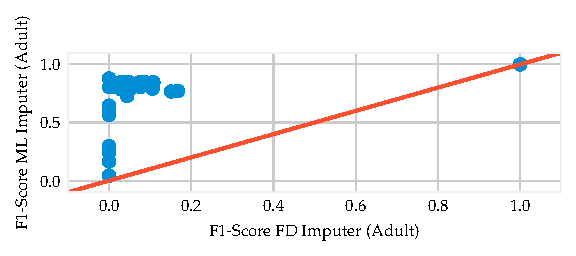
\includegraphics[width=\textwidth]{../figures/adult/f1_ml_fd}
     \caption{The figure compares the F1-Score of the FD Imputer compared to the F1-Score of ML Imputer. Each point represents one FD.}
     \label{fig:f1_ml_fd_adult}
 \end{figure}

However, for FDs where ML Imputer's scores are greater than 0.7, the FD Imputer's scores are greater than 0.
The two FDs for which the FD Imputer performs as well as the ML Imputer were identified and discussed in the previous sections.

\subsubsection{Overfitting ML Imputer}
In order to mimic the overfitting that takes place when FD Imputer looks up imputations on the train-set, it might be interesting to overfit ML Imputer models on purpose.
As shown in figure~\ref{fig:f1-ml-overfit-adult} and figure~\ref{fig:mse-ml-overfit-fractions}, neither the classifier-models, nor the regression-models trained by ML Imputer are capable of overfitting.
Future research-effort could be put into overfitting the models trained by ML Imputer with the goal of approximating the properties of FD Imputer.

\subsection{Dependency Detection with DepDetector}
The DepDetector algorithm was implemented to demonstrate dependency detection using models trained with ERM-strategies.
The `greedy' search-strategy was successfully used to detect minimal dependencies that are robust towards noise when used for training new models.
The dependencies detected this way are a blend of RFDs as discussed in the theory-section of this work.

Dependencies found with DepDetector can be used to save computation time when training a network for imputation.
Since minimal dependencies are often a subset of the whole relational instance, future imputation tasks can thus be performed more quickly by training models with less data.

Furthermore, minimal dependency detection helps explain the way a trained imputation-model works internally.
By reducing the amount of columns with which a model is trained, the way imputations are derived can often be reconstructed by inspecting the remaining columns.

It was not possible to derive FDs using ERM-strategies.
As discussed in the previous paragraphs, the behavior of FD Imputer might be approximated by overfitting models generated by ML Imputer.
In a future effort to derive robust FDs with DepDetector, it might be suitable to run the DepDetector-algorithm training overfitted models on purpose.

Computing results, especially using the `complete'-strategy, is computationally expensive.
Compared with FD detection algorithms, DepDetector is several orders of magnitude slower when detecting minimal dependencies.
For the Chess-dataset, the `complete'-strategy takes about \( 10^5 \) times longer until it converges, the `greedy'-strategy takes approximately \( 10^4 \) times longer.

DepDetector was implemented as a proof of concept.
There is a big margin for performance improvement.
Better performance can be achieved by training models on GPUs instead of CPUs.
Leveraging asynchronous programming techniques, models on the same level of the search lattice can be trained in parallel.
Furthermore, DepDetector internally models the search lattice as a tree rather than a lattice as in figure~\ref{fig:dep-detector-search-tree}.
This leads to redundant model training.

In general, the DepDetector approach is different from classical FD discovery algorithms in that minimal dependencies are detected solving an optimization problem on a graph.
The score of a parent-node has direct implications for the performance of its child-nodes.
Future research might investigate if this property is advantageous when searching for dependencies on big datasets.

\section{Conclusion}
In pursuit of identifying robust FDs, it is shown that FD Imputer can be used to measure robustness as defined in this work.
Experiments with FD Imputer lead to the conclusion that only FDs with RHSs containing classifiable data can be robust.
Generally, FDs are highly susceptible to noise in data.

A comparison between ML Imputer and FD Imputer suggests that imputation results yielded using FD Imputer are similar to using an overfitted model.
It is not possible to use FDs to impute continuous numerical data.

Dependencies with learned relaxation on the attribute comparison were successfully detected on datasets using machine learning techniques with an algorithm called DepDetector.
Two search-strategies were implemented and benchmarked on eight datasets.

\linespread{1}
\printbibliography % <---
\end{document}
